%% LyX 1.3 created this file.  For more info, see http://www.lyx.org/.
%% Do not edit unless you really know what you are doing.
\documentclass[english, 12pt]{article}
\usepackage{times}
%\usepackage{algorithm2e}
\usepackage{url}
\usepackage{bbm}
\usepackage[T1]{fontenc}
\usepackage[latin1]{inputenc}
\usepackage{geometry}
\geometry{verbose,letterpaper,tmargin=2cm,bmargin=2cm,lmargin=1.5cm,rmargin=1.5cm}
\usepackage{rotating}
\usepackage{color}
\usepackage{graphicx}
\usepackage{amsmath, amsthm, amssymb}
\usepackage{setspace}
\usepackage{lineno}
\usepackage{hyperref}
\usepackage{bbm}
\usepackage{makecell}
\usepackage{placeins}
\usepackage{subcaption}

%\renewcommand{\arraystretch}{1.8}

%\usepackage{xr}
%\externaldocument{SCT-supp}

%\linenumbers
%\doublespacing
\onehalfspacing
%\usepackage[authoryear]{natbib}
\usepackage{natbib} \bibpunct{(}{)}{;}{author-year}{}{,}

%Pour les rajouts
\usepackage{color}
\definecolor{trustcolor}{rgb}{0,0,1}

\usepackage{dsfont}
\usepackage[warn]{textcomp}
\usepackage{adjustbox}
\usepackage{multirow}
\usepackage{graphicx}
\graphicspath{{../figures/}}
\DeclareMathOperator*{\argmin}{\arg\!\min}

\let\tabbeg\tabular
\let\tabend\endtabular
\renewenvironment{tabular}{\begin{adjustbox}{max width=0.9\textwidth}\tabbeg}{\tabend\end{adjustbox}}

\makeatletter

%%%%%%%%%%%%%%%%%%%%%%%%%%%%%% LyX specific LaTeX commands.
%% Bold symbol macro for standard LaTeX users
%\newcommand{\boldsymbol}[1]{\mbox{\boldmath $#1$}}

%% Because html converters don't know tabularnewline
\providecommand{\tabularnewline}{\\}

\usepackage{babel}
\makeatother


\begin{document}

\renewcommand{\thefigure}{S\arabic{figure}}
\setcounter{figure}{0}
\renewcommand{\thetable}{S\arabic{table}}
\setcounter{table}{0}
\renewcommand{\theequation}{S\arabic{equation}}
\setcounter{equation}{0}

\section*{Quality control of summary statistics}

\begin{figure}[htbp]
	\centerline{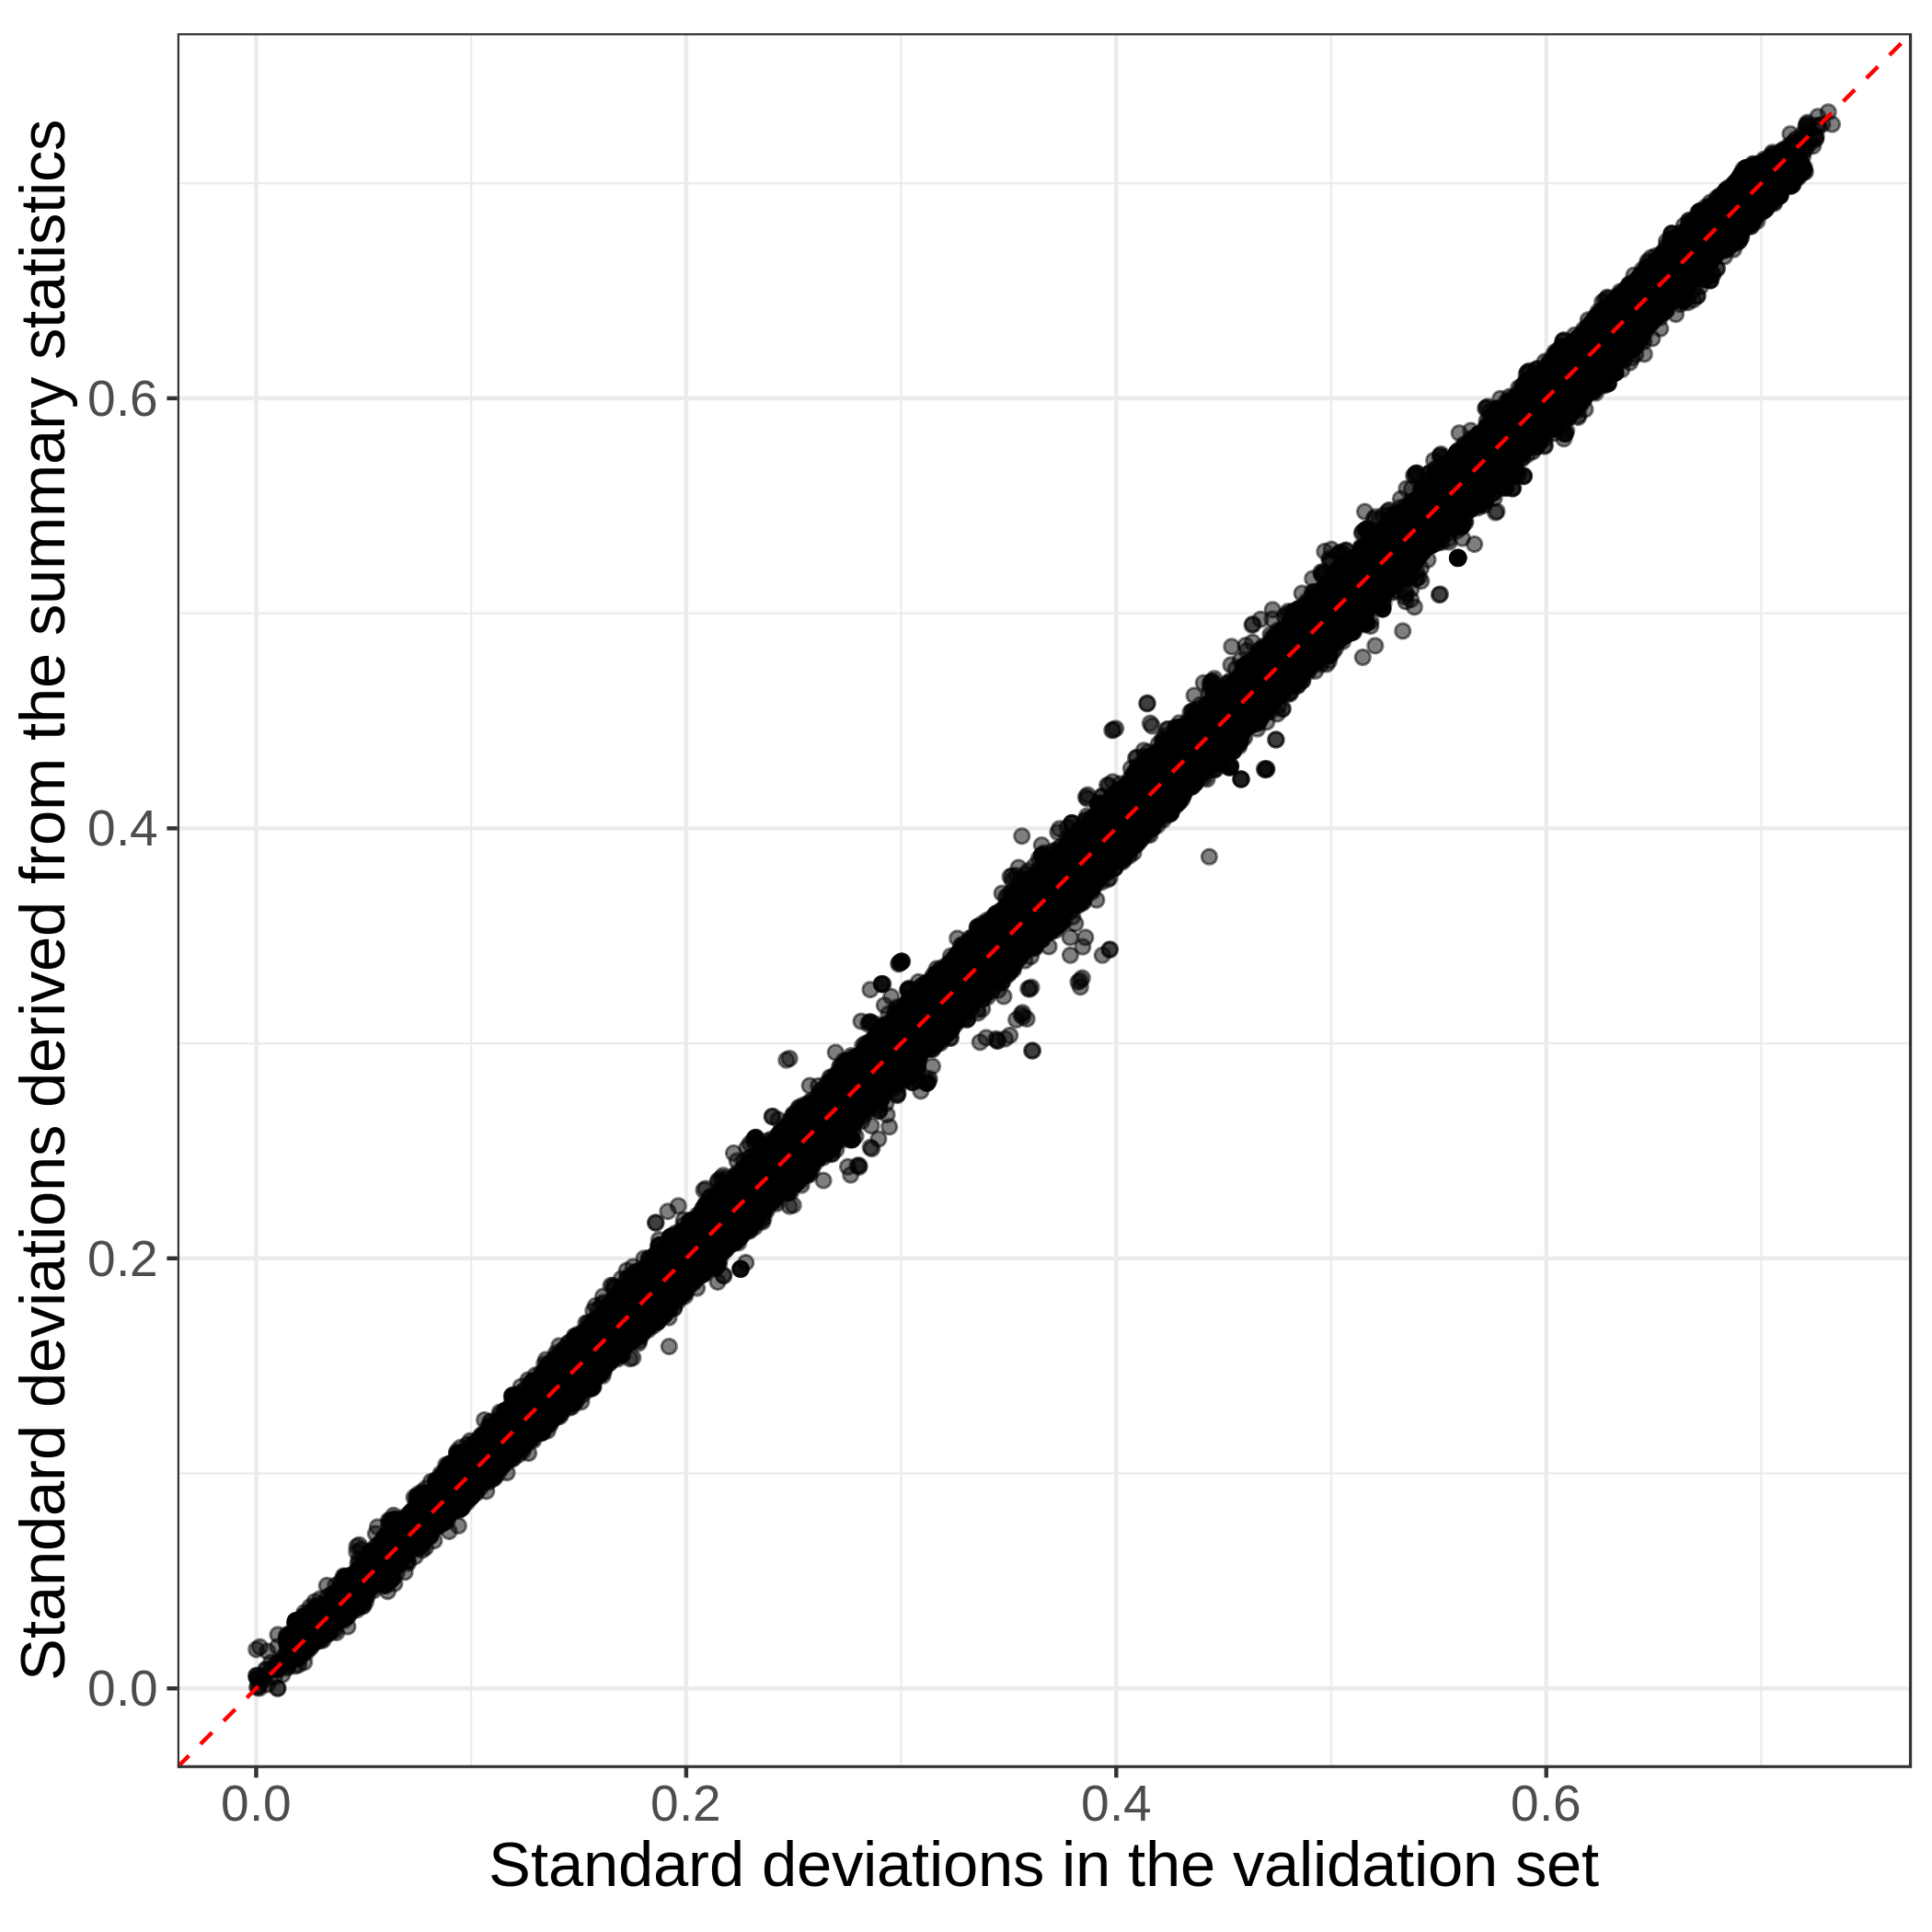
\includegraphics[width=0.7\textwidth]{sd-approx-simu}}
	\caption{In simulations, standard deviations derived from summary statistics based on equation \eqref{eq:approx-sd} versus the standard deviations of genotypes of individuals in the validation set.}
	\label{fig:sd-approx-simu}
\end{figure}

\begin{figure}[htbp]
	\centerline{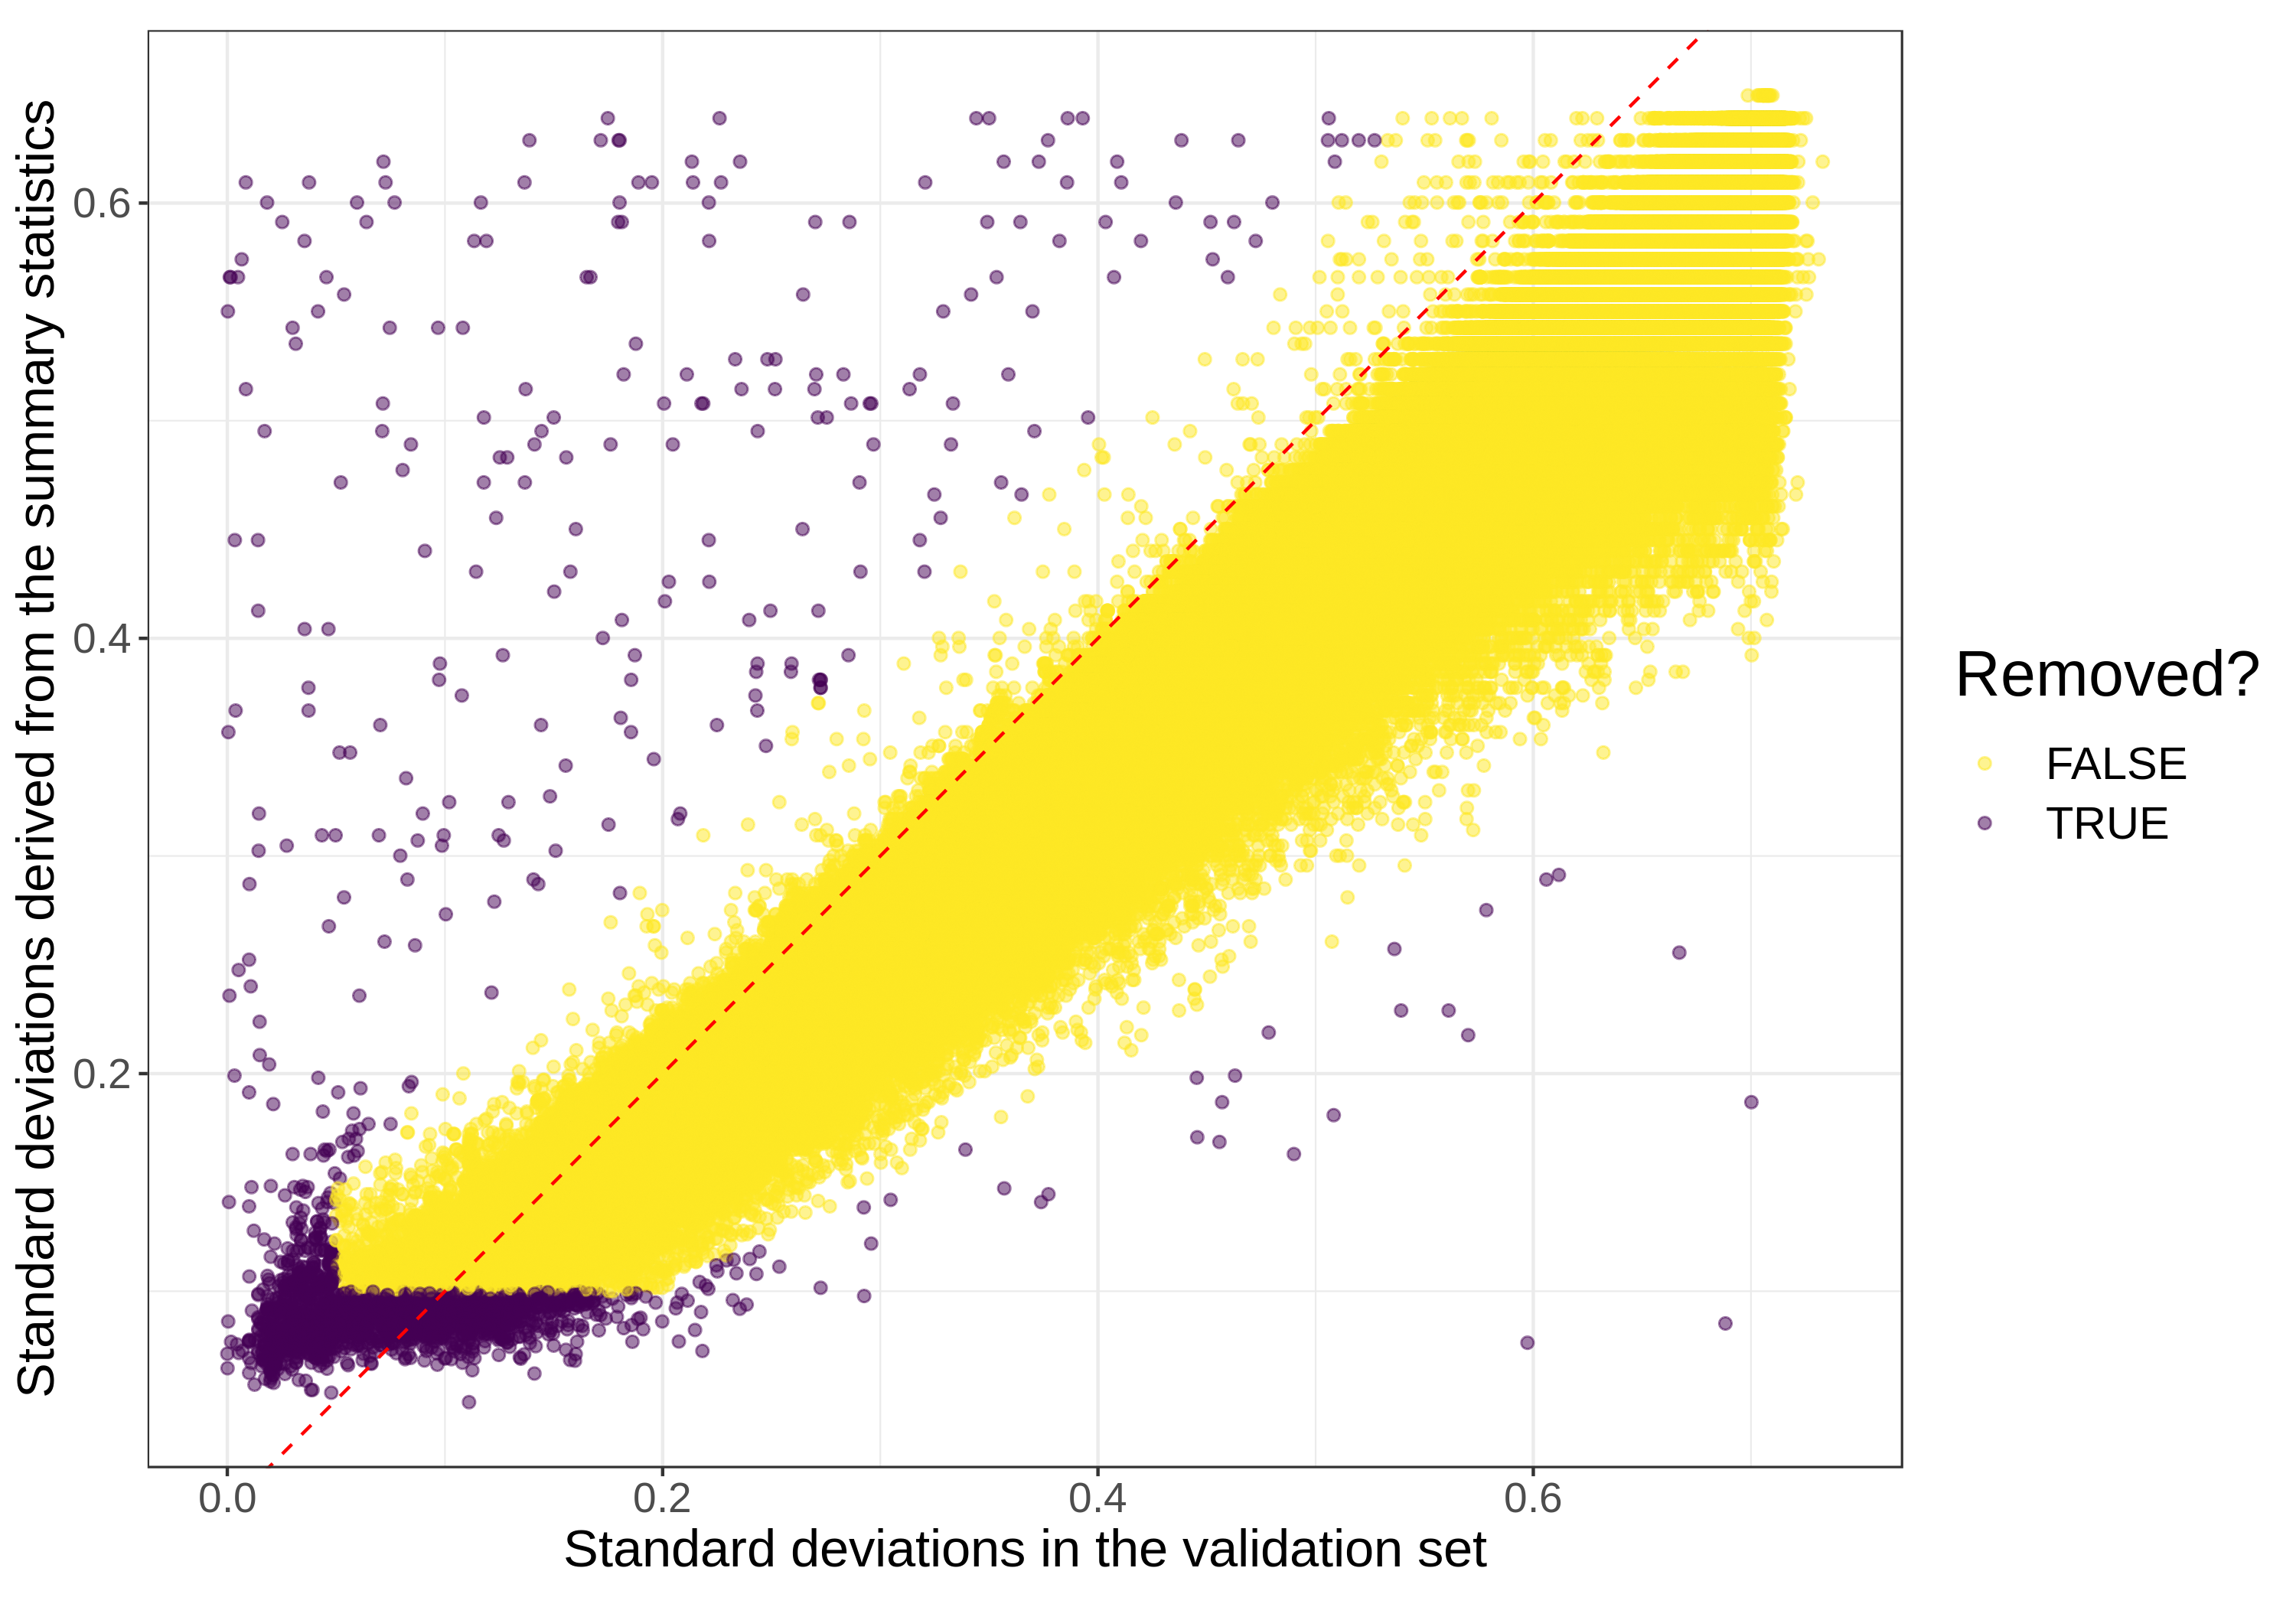
\includegraphics[width=0.9\textwidth]{sd-approx-BRCA}}
	\caption{Standard deviations derived from summary statistics of breast cancer based on equation \eqref{eq:approx-sd} versus the standard deviations of genotypes of individuals in the validation set. Coloring shows the quality control applied in this paper.}
	\label{fig:sd-approx-brca}
\end{figure}

\FloatBarrier

%%%%%%%%%%%%%%%%%%%%%%%%%%%%%%%%%%%%%%%%%%%%%%%%%%%%%%%%%%%%%%%%%%%%%%%%%%%%%%%%

\clearpage

\subsection*{Real data}

\begin{figure}[htb]
	\centerline{\includegraphics[width=0.85\textwidth]{AUC-auto}}
	\caption{}
	\label{fig:AUC-auto}
\end{figure}

\FloatBarrier

%%%%%%%%%%%%%%%%%%%%%%%%%%%%%%%%%%%%%%%%%%%%%%%%%%%%%%%%%%%%%%%%%%%%%%%%%%%%%%%%

\clearpage

\subsection*{Running LDpred2 per chromosome or genome-wide?}

\begin{figure}[htb]
	\centerline{\includegraphics[width=0.85\textwidth]{AUC-simu2-ldpred2}}
	\caption{}
	\label{fig:AUC-simu2-ldpred2}
\end{figure}

\begin{figure}[htb]
	\centerline{\includegraphics[width=0.85\textwidth]{AUC-real-ldpred2}}
	\caption{}
	\label{fig:AUC-real-ldpred2}
\end{figure}

\FloatBarrier

%%%%%%%%%%%%%%%%%%%%%%%%%%%%%%%%%%%%%%%%%%%%%%%%%%%%%%%%%%%%%%%%%%%%%%%%%%%%%%%%

\clearpage

\subsection*{Estimation of parameters in LDpred2}

\begin{figure}[htb]
	\centerline{\includegraphics[width=0.85\textwidth]{table_h2}}
	\caption{}
	\label{fig:TOCHANGE}
\end{figure}

\begin{figure}[htb]
	\centerline{\includegraphics[width=0.85\textwidth]{CAD-grid}}
	\caption{}
	\label{fig:CAD-grid}
\end{figure}


\begin{figure}[htb]
\begin{subfigure}[b]{\textwidth}
	\centerline{\includegraphics[width=0.8\textwidth]{CAD-auto}}
\end{subfigure}

\begin{subfigure}[b]{\textwidth}
	\centerline{\includegraphics[width=0.8\textwidth]{CAD-auto2}}
\end{subfigure}
\caption{}
\label{fig:CAD-auto}
\end{figure}

\FloatBarrier

%%%%%%%%%%%%%%%%%%%%%%%%%%%%%%%%%%%%%%%%%%%%%%%%%%%%%%%%%%%%%%%%%%%%%%%%%%%%%%%%

\end{document}
